\clearpage

\section{Month 2 - June}

\subsection{RAM speed, latency, and system cache}

Different RAM configurations result in different data access times, which could substantially influence the performance of large-scale computations. Generally, operations that involve a high volume of data access can be impacted by RAM speed and latency. We can see here the estimated latency for different RAM configurations:

\vspace{-1.5em}
\begin{equation*}
\begin{split}
    \text{Memory 3200 MHz, CL16:} & \quad \frac{16}{3200} \times 1000 \approx 5 \text{ ms} \\
    \text{Memory 4000 MHz, CL19:} & \quad \frac{19}{4000} \times 1000 \approx 4.75 \text{ ms} \\
    \text{Memory 2400 MHz, CL17:} & \quad \frac{17}{2400} \times 1000 \approx 7.08 \text{ ms} \\
\end{split}
\end{equation*}

Data needs to be fetched frequently from the RAM. If the RAM cannot supply data quickly enough, the CPU might have to wait for the data, leading to a memory bottleneck and a decrease in the overall performance.

In this context, the system's cache is also a key factor. The cache is a smaller, faster type of memory that stores copies of data from frequently used main memory locations. When the CPU needs data, it first looks for it in the cache (starting from L1, then L2, and finally L3). If the data is found there (a cache hit), it can be accessed much faster than from RAM. However, if the data is not in the cache (a cache miss), the CPU has to fetch it from RAM, which takes longer.

The efficiency of cache usage depends on many factors. One of them is data locality – if the data that needs to be accessed is stored close together, it's more likely to be loaded into the cache at the same time, increasing the chances of cache hits in the future. On the contrary, if data is scattered around, loading one piece of data into the cache is less likely to result in future cache hits.

\vspace{0.3em}

\begin{figure}[H]
	\centering
	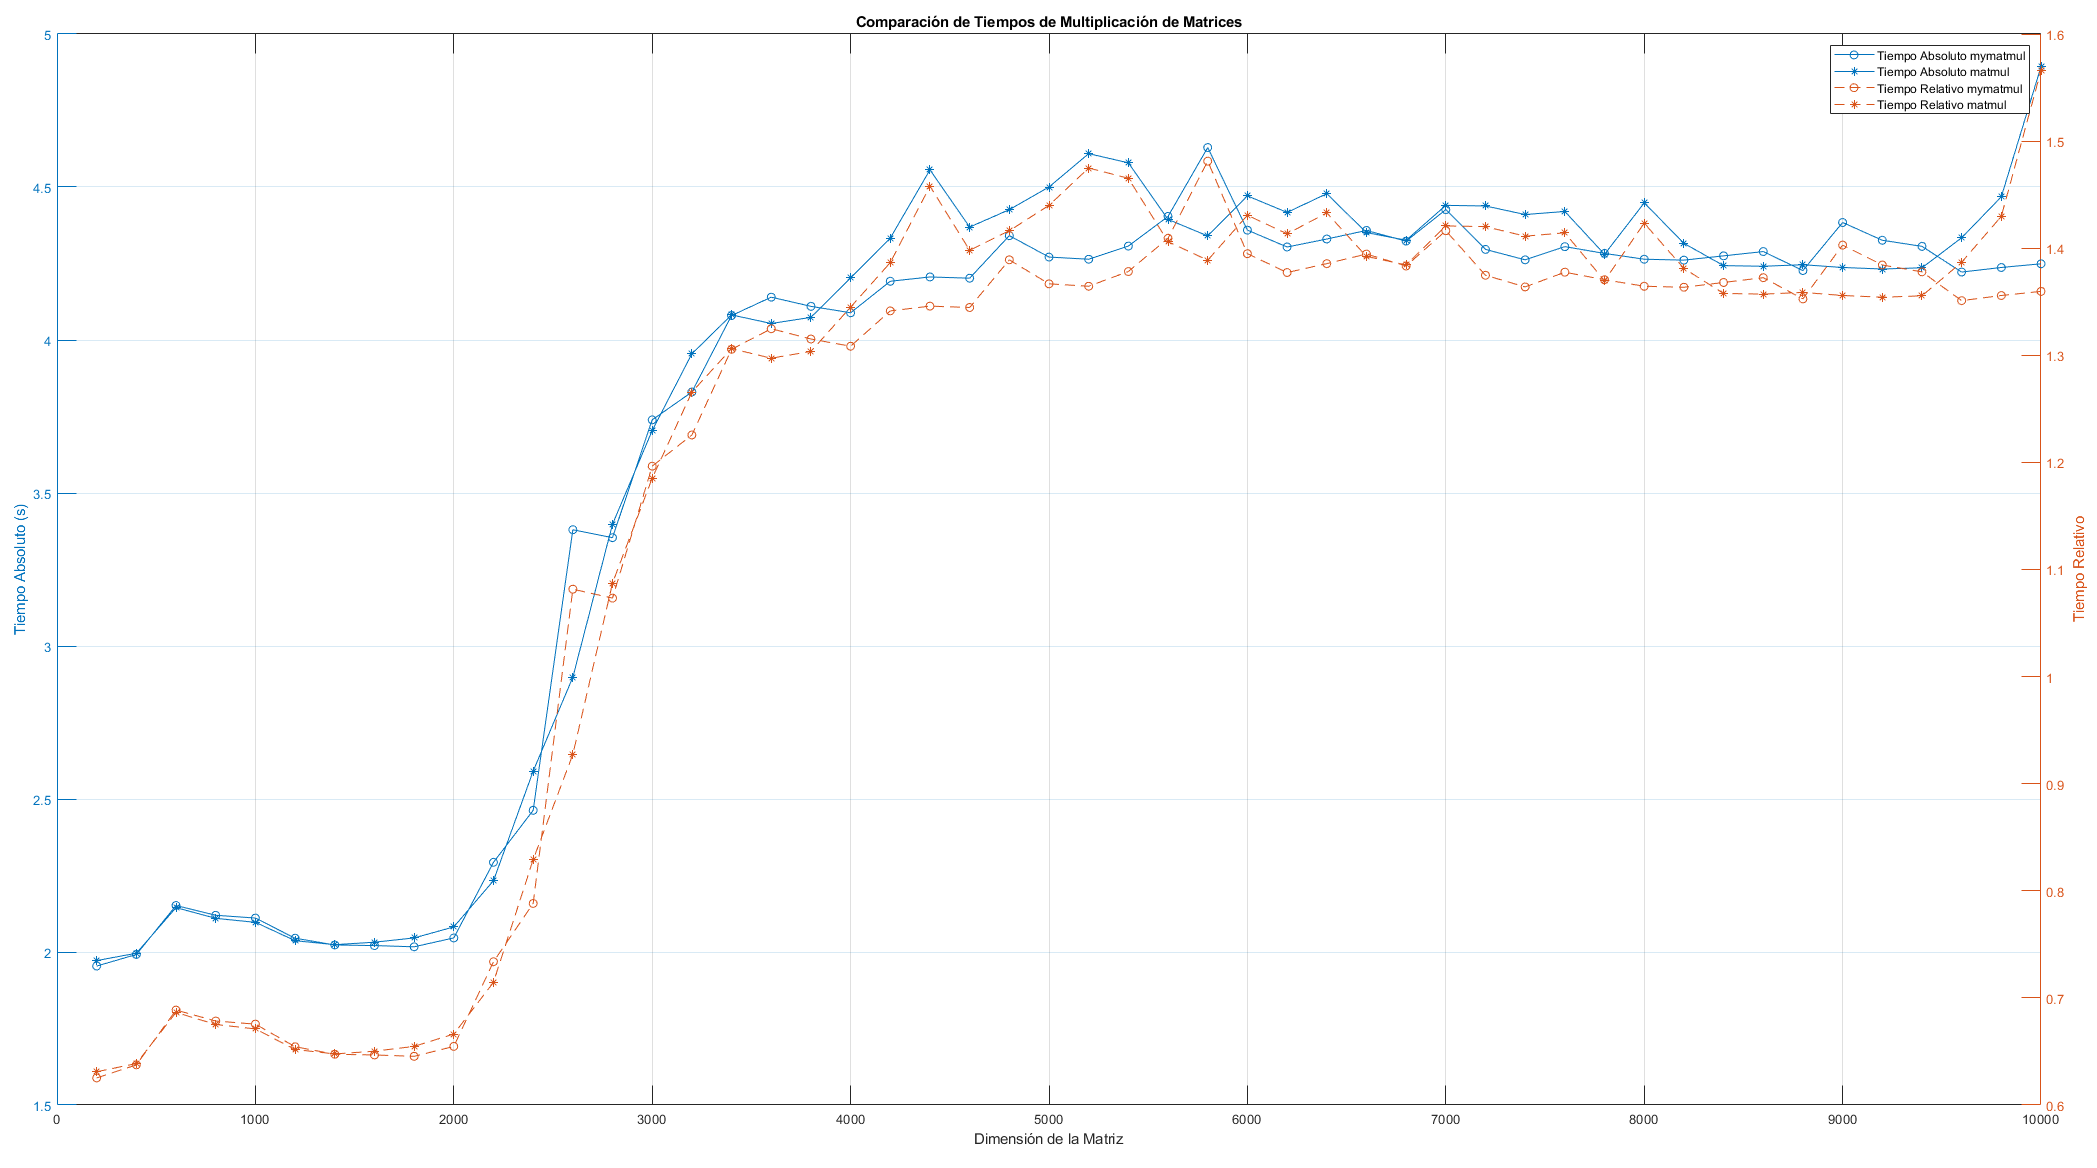
\includegraphics[width=103mm]{Figures/Imagenes/cache_problem.png}
   \caption{Cache memory without a good data locality}
\end{figure}

\clearpage


\subsection{Static vs Dynamic Variables}

When variables are declared as parameters, they are considered constant and occupy a fixed memory location. The Fortran compiler can often perform more aggressive optimizations on these variables since their values don't change at runtime.

Conversely, dynamically allocated variables are more flexible, but this can sometimes lead to less aggressive optimization since the compiler doesn't know the specifics about the memory layout and sizes until runtime.

For performance-critical code, it's generally beneficial to use static variables where possible.

\subsection{512-bit Vector Registers}

Modern CPUs have vector registers that allow for Single Instruction, Multiple Data (SIMD) operations. The 512-bit wide vector registers allow the CPU to perform arithmetic on multiple data points simultaneously, which can significantly speed up operations, especially in the context of matrix computations.

\subsection{Cache Blocking}

As discussed earlier, the processor cache is critical for performance. The cache stores copies of frequently accessed data, allowing the CPU to retrieve it faster compared to main memory. To efficiently utilize the cache, we implemented cache blocking in matrix multiplication. The idea is to divide the matrix into smaller blocks that fit into the cache, reducing the number of cache misses. 

\begin{lstlisting}
integer, parameter :: cacheSize = 32 * 1024 * 1024  ! 32MB
blockSize = int(sqrt(real(cacheSize) / 4.0))

do jj = 1, M, blockSize
    do ii = 1, N, blockSize
        do j = jj, min(jj + blockSize - 1, M)
            do i = ii, min(ii + blockSize - 1, N)
                b(i) = b(i) + A(i, j) * x(j)
            end do
        end do
    end do
end do
\end{lstlisting}


However, it is important to note that cache blocking alone still performs the matrix multiplication sequentially. This means that it only uses a single core of the CPU. In fact, using a single-threaded approach with cache blocking can sometimes result in worse performance compared to a simple matrix multiplication due to the additional loops and steps involved in handling the blocks. Therefore, while cache blocking is an essential optimization technique for reducing cache misses, the performance might still be suboptimal if the computation is not parallelized to take advantage of multiple cores.

\subsection{Thread vs Core Parallelism}

Threads are the smallest unit of processing that can be scheduled by an operating system. Core-level parallelism, on the other hand, refers to executing multiple tasks simultaneously on different physical cores of a processor.

Using threads is useful for hiding latency and is good for I/O bound tasks. Core-level parallelism is more suited for CPU-bound tasks, especially if the threads are not sharing data, as this can lead to a nearly linear speed-up.

\subsection{Parallelization with OpenMP}

To further optimize performance and overcome the limitations of the single-threaded approach, we introduced parallelization using OpenMP. This allows the matrix multiplication to be distributed across multiple CPU cores, greatly reducing the overall computation time.

In the code snippet below, we've combined cache blocking with parallelization. However, parallelizing the loops can introduce concurrency issues. One such issue is race conditions, which occur when multiple threads try to access and modify shared data simultaneously. This can lead to unpredictable and incorrect results.

To manage this, OpenMP provides a reduction clause. This clause ensures that each thread gets a private copy of the shared data, and after the threads have finished their computations, the private copies are combined into a single final result.

\begin{lstlisting}
!$omp parallel private(jj, ii, i, j) 
do jj = 1, M, blockSize
    do ii = 1, N, blockSize
        !$omp do reduction(+:b)
        do j = jj, min(jj + blockSize - 1, M)
            do i = ii, min(ii + blockSize - 1, N)
                b(i) = b(i) + A(i, j) * x(j)
            end do
        end do
        !$omp end do
    end do
end do
!$omp end parallel
\end{lstlisting}

\clearpage

Let's break down the code:

\begin{itemize}
    \item The outermost loops iterate over blocks of the matrix (`do jj = 1, M, blockSize` and `do ii = 1, N, blockSize`). 
    
    \item `!\$omp parallel private(jj, ii, i, j)` initiates a parallel region. The variables inside the private clause (`jj, ii, i, j`) are made private to each thread, meaning that each thread gets its own copy of these variables.
    
    \item `!\$omp do reduction(+:b)` indicates the start of the portion of code that should be executed in parallel by different threads. The reduction clause with the `+:b` operation specifies that we are performing a sum into the array `b`, and OpenMP should handle the reduction in a thread-safe way.
    
    \item The innermost loops (`do j = jj, min(jj + blockSize - 1, M)` and `do i = ii, min(ii + blockSize - 1, N)`) perform the actual multiplication and sum for each block. This part is similar to the standard matrix multiplication but operates on small blocks that fit into the cache.
    
    \item `!\$omp end do` and `!\$omp end parallel` mark the end of the parallel section.
\end{itemize}


With these optimizations, including cache blocking combined with parallelization, matrix-vector multiplication can be significantly accelerated, especially for large matrices where cache efficiency and parallel processing make a substantial difference.

